\documentclass[11pt,twocolumn]{article}

%==============================================================================
% PACKAGES
%==============================================================================
\usepackage[utf8]{inputenc}
\usepackage[T1]{fontenc}
\usepackage{mathptmx}
\usepackage{amsmath,amssymb,amsthm}
\usepackage{mathtools}
\usepackage{booktabs}
\usepackage{array}
\usepackage[margin=0.75in]{geometry}
\usepackage{fancyhdr}
\usepackage{hyperref}
\usepackage{xcolor}
\usepackage{float}
\usepackage{caption}
\usepackage{subcaption}
\usepackage{titlesec}
\usepackage{abstract}
\usepackage{enumitem}
\usepackage{tikz}
\usepackage{pgfplots}
\pgfplotsset{compat=1.17}
\usetikzlibrary{arrows.meta,positioning,calc,shapes,backgrounds}

%==============================================================================
% FORMATTING
%==============================================================================
\titlespacing*{\section}{0pt}{2.5ex}{1.5ex}
\titlespacing*{\subsection}{0pt}{2ex}{1ex}
\titlespacing*{\subsubsection}{0pt}{1.5ex}{0.5ex}
\setlist{nosep,leftmargin=1.5em}

% Colors
\definecolor{darkblue}{RGB}{0,51,102}
\definecolor{arxivblue}{RGB}{0,102,153}

% Hyperref
\hypersetup{
    colorlinks=true,
    linkcolor=darkblue,
    citecolor=darkblue,
    urlcolor=arxivblue,
    pdfauthor={Gregory John Komansky},
    pdftitle={A Graph-Theoretic Framework for DeFi Vault Risk Decomposition}
}

% Header
\pagestyle{fancy}
\fancyhf{}
\renewcommand{\headrulewidth}{0pt}
\fancyfoot[C]{\thepage}

% Theorem environments
\theoremstyle{plain}
\newtheorem{theorem}{Theorem}[section]
\newtheorem{lemma}[theorem]{Lemma}
\newtheorem{proposition}[theorem]{Proposition}
\newtheorem{corollary}[theorem]{Corollary}

\theoremstyle{definition}
\newtheorem{definition}[theorem]{Definition}
\newtheorem{example}[theorem]{Example}
\newtheorem{remark}[theorem]{Remark}

% Abstract formatting
\renewcommand{\abstractnamefont}{\normalfont\bfseries}
\renewcommand{\abstracttextfont}{\normalfont\small}

% Custom commands
\newcommand{\R}{\mathbb{R}}
\newcommand{\N}{\mathbb{N}}
\newcommand{\E}{\mathbb{E}}
\newcommand{\Var}{\text{Var}}
\newcommand{\bps}{\text{ bps}}
\DeclareMathOperator*{\argmax}{arg\,max}
\DeclareMathOperator*{\argmin}{arg\,min}

%==============================================================================
% TITLE
%==============================================================================
\title{\Large\bfseries A Graph-Theoretic Framework for\\DeFi Vault Risk Decomposition}

\author{
    Gregory John Komansky\thanks{Email: \texttt{gjkomansky@gmail.com}. The author thanks anonymous reviewers for valuable feedback. Data sources and replication code available at \url{https://github.com/eggbertgjk/vault-risk-framework}.}\\[0.3em]
    \small GJKapital Research
}

\date{\small January 2026\\[0.3em]\small\textit{Preliminary Draft --- Comments Welcome}}

%==============================================================================
% DOCUMENT
%==============================================================================
\begin{document}

\maketitle
\thispagestyle{fancy}

%------------------------------------------------------------------------------
% ABSTRACT
%------------------------------------------------------------------------------
\begin{onecolabstract}
Decentralized finance (DeFi) vaults---smart contracts that automate yield strategies across composable protocols---represent over \$16 billion in total value locked yet lack standardized risk decomposition frameworks. We propose a graph-theoretic approach: representing vaults as directed acyclic graphs where nodes are typed by four \textit{atomic primitives} (CONTRACT, ORACLE, GOVERNANCE, OPERATIONAL) and edges encode dependency relationships.

This formalization enables node-level risk attribution, where every basis point of expected loss traces to a specific primitive. We calibrate base rates from a dataset of 449 documented exploits (2016--2026) totaling \$15.7 billion in losses, sourced from DeFiLlama and validated against Rekt News.

Key finding: CONTRACT failures dominate frequency (65\%) while OPERATIONAL failures dominate severity (50\% of losses)---a distinction invisible without formal decomposition. The framework provides: (i) a complete taxonomy covering all historical exploit root causes, (ii) transparent aggregation from node-level to vault-level risk, and (iii) cross-protocol comparison on a common basis.

The framework does not predict exploits; rather, it provides the decomposition infrastructure that enables risk budgeting, concentration analysis, and board-level reporting---capabilities institutions require but DeFi currently lacks.

\vspace{0.8em}
\noindent\textbf{Keywords:} decentralized finance, risk decomposition, directed acyclic graphs, atomic primitives, smart contract risk, institutional allocation

\vspace{0.3em}
\noindent\textbf{JEL Classification:} G11, G21, G23, G32
\end{onecolabstract}

\vspace{1em}

%------------------------------------------------------------------------------
% 1. INTRODUCTION
%------------------------------------------------------------------------------
\section{Introduction}
\label{sec:intro}

\subsection{Motivation}

A fixed income portfolio manager can decompose bond portfolio risk into interpretable components: duration contribution, credit spread sensitivity, sector concentration, issuer limits. Every basis point of risk traces to a measurable factor. This decomposition infrastructure---developed over decades---enables institutional allocation, regulatory compliance, and fiduciary reporting.

No equivalent infrastructure exists for DeFi vaults.

Vaults are smart contracts that pool capital and execute yield-generating strategies across decentralized protocols. They have grown from negligible TVL in 2020 to over \$16 billion by late 2025 \cite{defillama2025}. Yet risk assessment remains primitive: audits verify code correctness but not architectural risk concentration; yield dashboards report APY but not expected loss; due diligence is ad hoc and incomparable across protocols.

This paper addresses a specific question: \textit{How should vault risk be decomposed to enable institutional-grade analysis?}

\subsection{Contribution}

We make three contributions:

\textbf{First}, we formalize vault risk decomposition. We represent vaults as directed acyclic graphs where nodes are typed by four \textit{atomic primitives}: CONTRACT, ORACLE, GOVERNANCE, and OPERATIONAL. We prove completeness---every exploit in our 449-incident dataset maps to these primitives. The formalization is not the novelty; the calibrated, auditable, standardized implementation is.

\textbf{Second}, we provide empirical calibration. Using 449 exploits totaling \$15.69B in losses over 9.56 years, we estimate base rates: CONTRACT failures occur at 6.11\% annually, OPERATIONAL at 1.93\%, ORACLE at 1.28\%, GOVERNANCE at 0.06\%. These are the first published base rates derived from comprehensive exploit data.

\textbf{Third}, we deliver decomposition infrastructure. The framework enables statements like: ``This vault's 45 bps expected loss decomposes as 22 bps CONTRACT, 12 bps OPERATIONAL, 8 bps ORACLE, 3 bps GOVERNANCE.'' This granularity enables risk budgeting, concentration limits, and comparable cross-protocol assessment---the factor-based analysis standard in traditional finance.

\subsection{Scope and Limitations}

We emphasize what this framework is \textit{not}. It is not an exploit predictor. Credit ratings do not predict which company will default; they categorize relative risk to enable portfolio decisions. Similarly, our framework categorizes architectural risk to enable allocation decisions.

The framework assesses \textit{on-chain} risk from observable properties (contract immutability, oracle redundancy, governance structure). Off-chain risks---custodial failures, social engineering, regulatory action---are outside scope.

Calibration derives from historical data. Novel attack vectors not represented in historical exploits may not be captured. Coefficients should be updated as new data accumulates.

\subsection{Related Work}

Our work intersects several literatures.

\textbf{DeFi Security.} Atzei et al.\ \cite{atzei2017} survey smart contract vulnerabilities. Perez and Livshits \cite{perez2019} analyze contract weaknesses at scale. Zhou et al.\ \cite{zhou2023sok} systematize DeFi attack knowledge. These works focus on vulnerability classification; we focus on risk aggregation for allocation decisions.

\textbf{Protocol Risk.} Gudgeon et al.\ \cite{gudgeon2020} analyze lending protocol stability. Werner et al.\ \cite{werner2022sok} systematize DeFi research. Qin et al.\ \cite{qin2022cefi} compare CeFi and DeFi risks. Our contribution is a formal aggregation framework, not protocol-specific analysis.

\textbf{AMM Theory.} Angeris and Chitra \cite{angeris2020} formalize constant function market makers. Milionis et al.\ \cite{milionis2022} analyze loss-versus-rebalancing. We incorporate AMM exposure as a dependency primitive.

\textbf{Traditional Risk.} Our approach draws on factor decomposition in fixed income \cite{litterman1991} and operational risk modeling \cite{basel2006}. The FMEA (Failure Mode and Effects Analysis) methodology from reliability engineering \cite{stamatis2003} informs our calibration approach.

\textbf{DeFi Risk Measurement.} Closest to our work, Xu and Livshits \cite{xu2022} propose a framework for quantifying DeFi protocol risk. Nexus Mutual \cite{nexusmutual2023} provides market-based risk pricing through parametric insurance. Artzner et al.\ \cite{artzner1999} establish coherent risk measure axioms that inform our aggregation design---our MAX propagation satisfies monotonicity and sub-additivity. Holló et al.\ \cite{hollo2012} construct the CISS composite indicator for systemic stress, whose aggregation methodology parallels our primitive-to-vault composition.

\subsection{Paper Structure}

Section \ref{sec:model} formalizes the vault graph model. Section \ref{sec:primitives} defines atomic primitives and proves completeness. Section \ref{sec:propagation} develops risk propagation. Section \ref{sec:calibration} presents empirical calibration. Section \ref{sec:application} demonstrates applications. Section \ref{sec:discussion} discusses limitations and extensions.

%------------------------------------------------------------------------------
% 2. THE VAULT GRAPH MODEL
%------------------------------------------------------------------------------
\section{The Vault Graph Model}
\label{sec:model}

\subsection{Preliminaries}

We represent a vault as a directed acyclic graph (DAG) capturing its dependency structure. Why a DAG? Figure \ref{fig:dag-comparison} illustrates:

\begin{figure}[H]
\centering
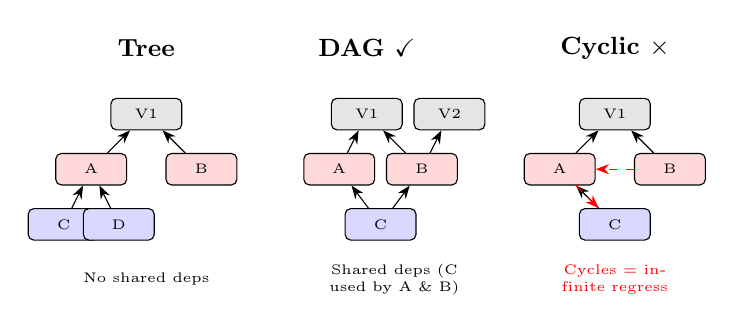
\begin{tikzpicture}[
    scale=0.7,
    every node/.style={font=\scriptsize},
    box/.style={rectangle, draw, rounded corners=2pt, minimum width=0.9cm, minimum height=0.4cm, font=\tiny},
]
    % TREE (left)
    \node[font=\small\bfseries] at (-4, 1.2) {Tree};
    \node[box, fill=gray!20] (t1) at (-4, 0) {V1};
    \node[box, fill=red!15] (t2) at (-5, -1) {A};
    \node[box, fill=red!15] (t3) at (-3, -1) {B};
    \node[box, fill=blue!15] (t4) at (-5.5, -2) {C};
    \node[box, fill=blue!15] (t5) at (-4.5, -2) {D};
    \draw[-{Stealth}] (t2) -- (t1);
    \draw[-{Stealth}] (t3) -- (t1);
    \draw[-{Stealth}] (t4) -- (t2);
    \draw[-{Stealth}] (t5) -- (t2);
    \node[font=\tiny, text width=2cm, align=center] at (-4, -3) {No shared deps};

    % DAG (center)
    \node[font=\small\bfseries] at (0, 1.2) {DAG \checkmark};
    \node[box, fill=gray!20] (d1) at (0, 0) {V1};
    \node[box, fill=gray!20] (d1b) at (1.5, 0) {V2};
    \node[box, fill=red!15] (d2) at (-0.5, -1) {A};
    \node[box, fill=red!15] (d3) at (1, -1) {B};
    \node[box, fill=blue!15] (d4) at (0.25, -2) {C};
    \draw[-{Stealth}] (d2) -- (d1);
    \draw[-{Stealth}] (d3) -- (d1);
    \draw[-{Stealth}] (d3) -- (d1b);
    \draw[-{Stealth}] (d4) -- (d2);
    \draw[-{Stealth}] (d4) -- (d3);
    \node[font=\tiny, text width=2.2cm, align=center] at (0.5, -3) {Shared deps (C used by A \& B)};

    % CYCLIC (right) - NOT ALLOWED
    \node[font=\small\bfseries] at (4.5, 1.2) {Cyclic $\times$};
    \node[box, fill=gray!20] (c1) at (4.5, 0) {V1};
    \node[box, fill=red!15] (c2) at (3.5, -1) {A};
    \node[box, fill=red!15] (c3) at (5.5, -1) {B};
    \node[box, fill=blue!15] (c4) at (4.5, -2) {C};
    \draw[-{Stealth}] (c2) -- (c1);
    \draw[-{Stealth}] (c3) -- (c1);
    \draw[-{Stealth}] (c4) -- (c2);
    \draw[-{Stealth}, red, dashed] (c2) -- (c4);
    \draw[-{Stealth}, red, dashed] (c3) -- (c2);
    \node[font=\tiny, text width=2cm, align=center, red] at (4.5, -3) {Cycles = infinite regress};
\end{tikzpicture}
\caption{Why DAG? Trees cannot represent shared dependencies (Chainlink used by multiple protocols). Cyclic graphs imply infinite capital regress. DAGs capture DeFi composability.}
\label{fig:dag-comparison}
\end{figure}

\noindent (i) \textit{Directed}: dependencies have direction---the vault depends on Morpho, not vice versa. (ii) \textit{Acyclic}: capital flows cannot cycle back to their origin in a single transaction (Lemma \ref{lem:acyclic}). (iii) \textit{Shared dependencies}: unlike trees, DAGs allow multiple protocols to share the same oracle (e.g., Chainlink).

\begin{definition}[Vault Graph]
\label{def:vault-graph}
A vault $V$ is represented by a tuple $G_V = (N, E, \tau, \omega)$ where:
\begin{itemize}
    \item $N$ is a finite set of nodes
    \item $E \subseteq N \times N$ is a set of directed edges
    \item $\tau: N \rightarrow \mathcal{P}$ assigns each node a primitive type
    \item $\omega: N \rightarrow \R^k$ assigns each node a property vector
\end{itemize}
where $\mathcal{P} = \{\texttt{CONTRACT}, \texttt{ORACLE}, \texttt{GOVERNANCE}, \texttt{OPERATIONAL}\}$ is the set of primitive types.\footnote{Our taxonomy consolidates related failure modes. CONTRACT captures smart contract logic bugs, reentrancy, and access control errors. OPERATIONAL captures infrastructure failures, key compromises, and bridge exploits. This yields categories that are both exhaustive and mutually exclusive for allocation purposes.}
\end{definition}

Edges encode dependency: $(n_i, n_j) \in E$ indicates that node $n_j$ depends on node $n_i$. Failure of $n_i$ may propagate to $n_j$.

\begin{definition}[Dependency]
Node $n_j$ \textit{depends on} node $n_i$, written $n_i \prec n_j$, if there exists a directed path from $n_i$ to $n_j$ in $G_V$.
\end{definition}

\begin{lemma}[Acyclicity]
\label{lem:acyclic}
For any vault with well-defined capital flows, $G_V$ is acyclic.
\end{lemma}

\begin{proof}
Suppose $G_V$ contains a cycle $n_1 \to n_2 \to \cdots \to n_k \to n_1$. Each edge represents dependency: $n_{i+1}$ requires $n_i$ to function. A cycle implies $n_1$ requires itself through intermediaries---an infinite regress. Since vaults execute finite transactions returning value to depositors, such cycles cannot exist. Thus $G_V$ is a DAG.
\end{proof}

Acyclicity ensures well-defined topological ordering, enabling bottom-up risk aggregation.

\subsection{Graph Structure}

Vaults exhibit layered structure reflecting DeFi composability:

\begin{example}[Morpho Vault Structure]
\label{ex:morpho}
A Morpho USDC vault has approximate structure:
\begin{center}
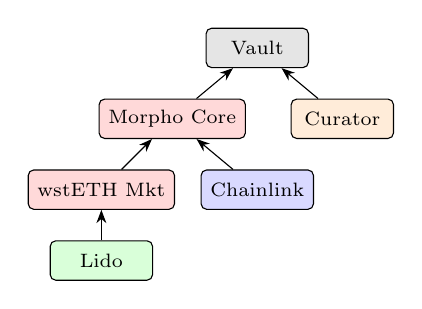
\begin{tikzpicture}[
    scale=0.9,
    every node/.style={font=\small},
    box/.style={rectangle, draw, rounded corners=2pt, minimum width=1.3cm, minimum height=0.5cm, font=\scriptsize},
    contract/.style={box, fill=red!15},
    oracle/.style={box, fill=blue!15},
    governance/.style={box, fill=orange!15},
    operational/.style={box, fill=green!15},
]
    % Layer 0: Vault
    \node[box, fill=gray!20] (vault) at (0,0) {Vault};

    % Layer 1: Direct dependencies
    \node[contract] (morpho) at (-1.2,-1) {Morpho Core};
    \node[governance] (curator) at (1.2,-1) {Curator};

    % Layer 2: Morpho's dependencies
    \node[contract] (market) at (-2.2,-2) {wstETH Mkt};
    \node[oracle] (oracle) at (0,-2) {Chainlink};

    % Layer 3: Market's dependencies
    \node[operational] (lido) at (-2.2,-3) {Lido};

    % Edges (dependency flows upward)
    \draw[-{Stealth}] (morpho) -- (vault);
    \draw[-{Stealth}] (curator) -- (vault);
    \draw[-{Stealth}] (market) -- (morpho);
    \draw[-{Stealth}] (oracle) -- (morpho);
    \draw[-{Stealth}] (lido) -- (market);
\end{tikzpicture}
\end{center}
Each node has type $\tau(n) \in \mathcal{P}$ and properties $\omega(n)$. Arrows indicate dependency: the vault depends on Morpho Core, which depends on the wstETH market, which depends on Lido.
\end{example}

%------------------------------------------------------------------------------
% 3. ATOMIC PRIMITIVES
%------------------------------------------------------------------------------
\section{Atomic Risk Primitives}
\label{sec:primitives}

\subsection{Why Four Primitives?}

A natural question: why four categories, not ten or two? The taxonomy emerged empirically from categorizing 449 exploits by root cause technique, subject to three constraints:

\textbf{Mutual exclusivity.} Each exploit maps to exactly one root cause. When an oracle manipulation enables a contract exploit, we attribute to the \textit{initial} failure (oracle), not the downstream consequence.

\textbf{Collective exhaustiveness.} The four categories cover 448 of 449 exploits (99.8\%). One ECONOMIC incident (\$0.34M, stablecoin depeg) was excluded as de minimis and arguably belongs to DEPENDENCY risk of underlying assets.

\textbf{Actionable distinctness.} Each category has different mitigations: CONTRACT risk is addressed by audits, immutability, and formal verification; ORACLE risk by source redundancy and TWAP designs; GOVERNANCE risk by timelocks and multisig requirements; OPERATIONAL risk by cold storage and MPC key management. Categories with identical mitigations should merge; these four do not.

We considered finer granularity (e.g., separating reentrancy from access control within CONTRACT) but this reduces statistical power per category---GOVERNANCE already has only 3 incidents. We considered coarser granularity (e.g., merging ORACLE into CONTRACT) but this obscures actionable distinctions: oracle redundancy does not help contract bugs.

\subsection{Primitive Definitions}

We define the four atomic primitive classes. For each primitive, we specify properties that: (i) are observable on-chain or from public sources, (ii) have documented or plausible relationship to failure rates, and (iii) are actionable for risk assessment. The property lists are illustrative, not exhaustive---practitioners may add domain-specific properties.

\begin{definition}[CONTRACT Primitive]
A \texttt{CONTRACT} node represents smart contract logic risk: bugs, reentrancy, access control errors, overflow/underflow, and flashloan exploits. This is the dominant failure mode (292 of 449 exploits, 65\%). Properties include:
\begin{itemize}
    \item \texttt{immutable} $\in \{0,1\}$: whether code can be upgraded
    \item \texttt{audit\_count} $\in \N$: number of independent security audits
    \item \texttt{tvl\_days} $\in \R^+$: cumulative $\sum_t \text{TVL}_t$ (Lindy proxy---the longer a protocol survives with high TVL, the longer it is expected to survive, per the Lindy effect \cite{taleb2012})
    \item \texttt{complexity} $\in \R^+$: lines of code or cyclomatic complexity
\end{itemize}
\end{definition}

\begin{definition}[ORACLE Primitive]
An \texttt{ORACLE} node represents price feed risk: manipulation, stale data, single-source failures. (61 of 449 exploits, 14\%). Properties include:
\begin{itemize}
    \item \texttt{type} $\in \{\text{chainlink}, \text{twap}, \text{custom}\}$
    \item \texttt{sources} $\in \N$: number of independent data sources
    \item \texttt{heartbeat} $\in \R^+$: maximum staleness (seconds)
    \item \texttt{deviation} $\in (0,1)$: update trigger threshold
\end{itemize}
\end{definition}

\begin{definition}[GOVERNANCE Primitive]
A \texttt{GOVERNANCE} node represents administrative control risk: rug pulls, malicious upgrades, governance attacks. (3 of 449 exploits---see Remark \ref{rem:gov-bayes} on small-sample estimation). Properties include:
\begin{itemize}
    \item \texttt{type} $\in \{\text{eoa}, \text{multisig}, \text{timelock}, \text{dao}\}$
    \item \texttt{threshold}: $m$-of-$n$ requirement (for multisig)
    \item \texttt{delay} $\in \R^+$: timelock duration (seconds)
\end{itemize}
\end{definition}

\begin{definition}[OPERATIONAL Primitive]
An \texttt{OPERATIONAL} node represents infrastructure risk: private key compromises, bridge failures, frontend attacks, DNS hijacking. (92 of 449 exploits, 20\%, highest losses at \$7.8B). Properties include:
\begin{itemize}
    \item \texttt{key\_management} $\in \{\text{hot}, \text{cold}, \text{mpc}, \text{hsm}\}$
    \item \texttt{bridge} $\in \{0,1\}$: whether cross-chain bridge involved
    \item \texttt{frontend\_security}: DNS, hosting, CDN configuration
\end{itemize}
\end{definition}

\subsection{Completeness}

\begin{theorem}[Primitive Completeness]
\label{thm:complete}
Every exploit in our dataset of 449 DeFi incidents maps to failure in at least one primitive class.
\end{theorem}

\begin{proof}
We categorized each exploit by root cause using keyword matching on technique descriptions, validated by manual review. The categorization from our dataset of 449 DeFi exploits:
\begin{itemize}
    \item \texttt{CONTRACT}: Logic bugs, reentrancy, access control, flashloan exploits---292 incidents (\$6.99B)
    \item \texttt{OPERATIONAL}: Key compromise, bridge failures, infrastructure attacks---92 incidents (\$7.82B)
    \item \texttt{ORACLE}: Price manipulation, stale data, single-source failure---61 incidents (\$0.69B)
    \item \texttt{GOVERNANCE}: Rug pulls, malicious upgrades, admin key abuse---3 incidents (\$0.19B)
\end{itemize}
One ECONOMIC incident (\$0.34M, depeg-related) excluded as de minimis. Total: 449 exploits, \$15.69B losses. Date range: 2016-06-17 to 2026-01-06. Categorization code and full dataset available in supplementary materials.
\end{proof}

\begin{remark}
Some exploits involve multiple primitives (e.g., oracle manipulation enabling contract exploit). We attribute to the \textit{root cause} primitive---the initial failure that enabled the attack chain.
\end{remark}

\begin{remark}[GOVERNANCE Base Rate]
\label{rem:gov-bayes}
With only $n=3$ GOVERNANCE exploits, the frequentist point estimate $\hat{r}_{\texttt{GOV}}^{(0)} = 3/(500 \times 9.56) = 0.06\%$ has wide confidence intervals. We interpret this as an order-of-magnitude bound rather than a precise estimate. A Bayesian treatment with uninformative prior $\text{Beta}(1,1)$ and $N \cdot T = 4{,}780$ protocol-years yields posterior $\text{Beta}(4, 4777)$, giving a 95\% credible interval of $[0.02\%, 0.21\%]$. The low rate is consistent with governance attacks being genuinely rare (protocols with EOA admin keys are quickly exploited and exit the sample, while protocols with timelocks and multisigs are harder to attack). We retain the point estimate for computational convenience but flag the uncertainty.
\end{remark}

%------------------------------------------------------------------------------
% 4. RISK PROPAGATION
%------------------------------------------------------------------------------
\section{Risk Propagation and Aggregation}
\label{sec:propagation}

\subsection{Node-Level Risk}

Each node $n$ has intrinsic risk determined by its type and properties.

\begin{definition}[Node Risk Function]
For node $n$ with type $\tau(n) = p$ and property vector $\omega(n) = \mathbf{x}$:
\begin{equation}
\label{eq:node-risk}
r(n) = r_p^{(0)} \cdot \prod_{j=1}^{k} (1 + \beta_{p,j} \cdot x_j)
\end{equation}
where $r_p^{(0)}$ is the base rate for primitive $p$ and $\beta_{p,j}$ is the adjustment coefficient for property $j$.
\end{definition}

Figure \ref{fig:node-risk} illustrates this multiplicative adjustment.

\begin{figure}[H]
\centering
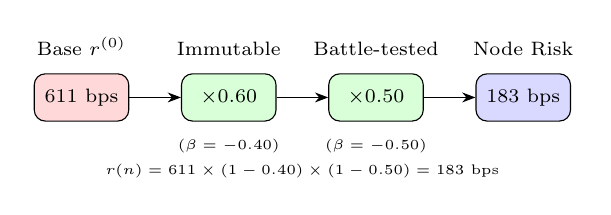
\begin{tikzpicture}[scale=0.85, every node/.style={font=\scriptsize}]
    % Base rate box
    \node[draw, fill=red!15, minimum width=1.2cm, minimum height=0.6cm, rounded corners] (base) at (0,0) {611 bps};
    \node[above=0.1cm of base] {Base $r^{(0)}$};

    % Multiplier 1
    \node[draw, fill=green!15, minimum width=1.2cm, minimum height=0.6cm, rounded corners] (m1) at (2.2,0) {$\times 0.60$};
    \node[above=0.1cm of m1] {Immutable};
    \node[below=0.1cm of m1, font=\tiny] {($\beta=-0.40$)};

    % Multiplier 2
    \node[draw, fill=green!15, minimum width=1.2cm, minimum height=0.6cm, rounded corners] (m2) at (4.4,0) {$\times 0.50$};
    \node[above=0.1cm of m2] {Battle-tested};
    \node[below=0.1cm of m2, font=\tiny] {($\beta=-0.50$)};

    % Result
    \node[draw, fill=blue!15, minimum width=1.2cm, minimum height=0.6cm, rounded corners] (result) at (6.6,0) {183 bps};
    \node[above=0.1cm of result] {Node Risk};

    % Arrows
    \draw[-{Stealth}] (base) -- (m1);
    \draw[-{Stealth}] (m1) -- (m2);
    \draw[-{Stealth}] (m2) -- (result);

    % Formula below
    \node[font=\tiny] at (3.3,-1.1) {$r(n) = 611 \times (1-0.40) \times (1-0.50) = 183$ bps};
\end{tikzpicture}
\caption{Node Risk Function: Multiplicative adjustments from base rate. Each property scales the previous result, ensuring non-negativity.}
\label{fig:node-risk}
\end{figure}

\textbf{Why multiplicative?} We choose the multiplicative form over additive ($r_p^{(0)} + \sum \beta_j x_j$) for three reasons: (i) \textit{non-negativity}---risk cannot go negative regardless of how many mitigants are stacked; (ii) \textit{interpretability}---$\beta = -0.4$ means ``40\% risk reduction,'' matching how practitioners describe audit impact; (iii) \textit{diminishing returns}---the second audit reduces less absolute risk than the first, reflecting empirical observation that marginal security investment has decreasing returns. An additive form would allow negative risk and imply constant marginal returns, both unrealistic.

\subsection{Risk Propagation}

Risk propagates upward through the dependency graph.

\begin{definition}[Propagated Risk]
For node $n$ with parent set $\text{Pa}(n) = \{m : (m,n) \in E\}$:
\begin{equation}
\label{eq:propagation}
R(n) = r(n) + \max_{m \in \text{Pa}(n)} \bigl\{ \gamma_{m \to n} \cdot R(m) \bigr\}
\end{equation}
where $\gamma_{m \to n} \in [0,1]$ is the propagation coefficient from $m$ to $n$, and $R(m)$ is computed recursively with base case $R(m) = r(m)$ for leaf nodes.

\textbf{Why $\gamma \in [0,1]$?} The propagation coefficient represents the fraction of dependency risk that transmits to the dependent node. $\gamma = 1$ means full transmission (if Lido fails, the wstETH market loses everything). $\gamma < 1$ means partial transmission (the vault has other collateral types, so Lido failure causes partial, not total, loss). $\gamma > 1$ (amplification) is theoretically possible in leveraged structures but rare in practice; we constrain to $[0,1]$ for parsimony. Default: $\gamma = 1$ unless the dependent node has documented redundancy.
\end{definition}

\begin{remark}
We use $\max$ rather than $\sum$ because a single critical dependency failure is typically sufficient for loss. This follows the ``weakest link'' model in reliability engineering. For portfolios of independent vaults, risks would sum; within a single vault's dependency chain, the binding constraint dominates.
\end{remark}

Figure \ref{fig:propagation} illustrates risk propagation with concrete values.

\begin{figure}[H]
\centering
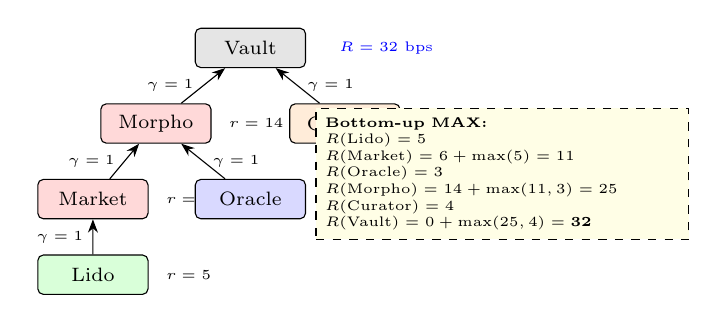
\begin{tikzpicture}[
    scale=0.8,
    every node/.style={font=\scriptsize},
    box/.style={rectangle, draw, rounded corners=2pt, minimum width=1.4cm, minimum height=0.5cm},
]
    % Vault (top)
    \node[box, fill=gray!20] (vault) at (0,0) {Vault};
    \node[right=0.3cm of vault, font=\tiny, blue] {$R=32$ bps};

    % Layer 1
    \node[box, fill=red!15] (morpho) at (-1.5,-1.2) {Morpho};
    \node[right=0.1cm of morpho, font=\tiny] {$r=14$};
    \node[box, fill=orange!15] (curator) at (1.5,-1.2) {Curator};
    \node[right=0.1cm of curator, font=\tiny] {$r=4$};

    % Layer 2
    \node[box, fill=red!15] (market) at (-2.5,-2.4) {Market};
    \node[right=0.1cm of market, font=\tiny] {$r=6$};
    \node[box, fill=blue!15] (oracle) at (0,-2.4) {Oracle};
    \node[right=0.1cm of oracle, font=\tiny] {$r=3$};

    % Layer 3
    \node[box, fill=green!15] (lido) at (-2.5,-3.6) {Lido};
    \node[right=0.1cm of lido, font=\tiny] {$r=5$};

    % Edges with gamma values
    \draw[-{Stealth}] (morpho) -- node[left, font=\tiny] {$\gamma=1$} (vault);
    \draw[-{Stealth}] (curator) -- node[right, font=\tiny] {$\gamma=1$} (vault);
    \draw[-{Stealth}] (market) -- node[left, font=\tiny] {$\gamma=1$} (morpho);
    \draw[-{Stealth}] (oracle) -- node[right, font=\tiny] {$\gamma=1$} (morpho);
    \draw[-{Stealth}] (lido) -- node[left, font=\tiny] {$\gamma=1$} (market);

    % Calculation box
    \node[draw, dashed, fill=yellow!10, text width=4.5cm, font=\tiny, align=left] at (4,-2) {
        \textbf{Bottom-up MAX:}\\
        $R(\text{Lido}) = 5$\\
        $R(\text{Market}) = 6 + \max(5) = 11$\\
        $R(\text{Oracle}) = 3$\\
        $R(\text{Morpho}) = 14 + \max(11,3) = 25$\\
        $R(\text{Curator}) = 4$\\
        $R(\text{Vault}) = 0 + \max(25,4) = \mathbf{32}$
    };
\end{tikzpicture}
\caption{Risk Propagation: MAX aggregation from leaf nodes upward. Vault risk (32 bps) is dominated by the Morpho $\to$ Market $\to$ Lido critical path.}
\label{fig:propagation}
\end{figure}

\subsection{Vault-Level Aggregation}

\begin{definition}[Vault Risk Score]
For vault $V$ with graph $G_V$, let $\text{Roots}(G_V)$ be the set of root nodes (nodes with no outgoing edges---typically the vault contract itself). The vault risk score is:
\begin{equation}
\label{eq:vrs}
\text{VRS}(V) = \sum_{n \in \text{Roots}(G_V)} w_n \cdot R(n)
\end{equation}
where $w_n$ is the exposure weight (e.g., allocation fraction) to root $n$.
\end{definition}

For single-root vaults (the typical case), $\text{VRS}(V) = R(\text{root})$.

\subsection{Attribution}

The framework produces node-level attribution:

\begin{definition}[Risk Attribution]
The risk contribution of node $n$ to vault $V$ is:
\begin{equation}
\text{Attr}(n, V) = r(n) \cdot \mathbf{1}[n \text{ on critical path}]
\end{equation}
where the critical path is the dependency chain with maximum propagated risk.
\end{definition}

This enables statements like: ``14 bps from Morpho Core (CONTRACT), 6 bps from wstETH market (CONTRACT), 5 bps from Lido (OPERATIONAL---external protocol dependency), 3 bps from Chainlink (ORACLE), 4 bps from curator multisig (GOVERNANCE). Total: 32 bps.''

\subsection{From VRS to Expected Annual Loss (EAL)}

The Vault Risk Score (VRS) measures annualized failure probability. To convert to dollar-denominated \textit{Expected Annual Loss} (EAL), we incorporate severity and exposure:

\begin{definition}[Expected Annual Loss]
For vault $V$ with TVL (total value locked) $L$:
\begin{equation}
\label{eq:eal}
\text{EAL}(V) = \sum_{p \in \mathcal{P}} \text{VRS}_p(V) \cdot s_p \cdot L
\end{equation}
where $\text{VRS}_p(V)$ is the vault's risk score attributed to primitive $p$, and $s_p \in [0,1]$ is the severity (loss-given-failure) for primitive $p$.
\end{definition}

Figure \ref{fig:eal} illustrates how EAL converts probability to dollar-denominated loss.

\begin{figure}[H]
\centering
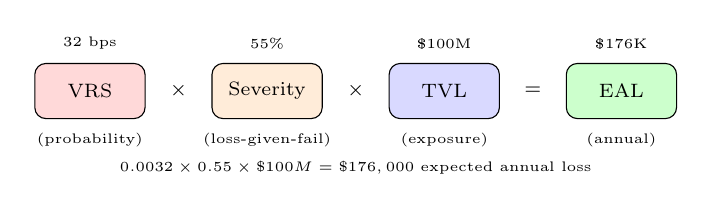
\begin{tikzpicture}[scale=0.75, every node/.style={font=\scriptsize}]
    % VRS box
    \node[draw, fill=red!15, minimum width=1.4cm, minimum height=0.7cm, rounded corners] (vrs) at (0,0) {VRS};
    \node[above=0.05cm of vrs, font=\tiny] {32 bps};
    \node[below=0.05cm of vrs, font=\tiny] {(probability)};

    % Times symbol
    \node at (1.5, 0) {$\times$};

    % Severity box
    \node[draw, fill=orange!15, minimum width=1.4cm, minimum height=0.7cm, rounded corners] (sev) at (3,0) {Severity};
    \node[above=0.05cm of sev, font=\tiny] {55\%};
    \node[below=0.05cm of sev, font=\tiny] {(loss-given-fail)};

    % Times symbol
    \node at (4.5, 0) {$\times$};

    % TVL box
    \node[draw, fill=blue!15, minimum width=1.4cm, minimum height=0.7cm, rounded corners] (tvl) at (6,0) {TVL};
    \node[above=0.05cm of tvl, font=\tiny] {\$100M};
    \node[below=0.05cm of tvl, font=\tiny] {(exposure)};

    % Equals
    \node at (7.5, 0) {$=$};

    % EAL result
    \node[draw, fill=green!20, minimum width=1.4cm, minimum height=0.7cm, rounded corners] (eal) at (9,0) {EAL};
    \node[above=0.05cm of eal, font=\tiny] {\$176K};
    \node[below=0.05cm of eal, font=\tiny] {(annual)};

    % Formula
    \node[font=\tiny] at (4.5, -1.3) {$0.0032 \times 0.55 \times \$100M = \$176,000$ expected annual loss};
\end{tikzpicture}
\caption{EAL Calculation: Vault Risk Score (probability) $\times$ Severity (loss-given-failure) $\times$ TVL (exposure) = Expected Annual Loss in dollars.}
\label{fig:eal}
\end{figure}

Severity captures that not all failures result in total loss. From our calibration:

\begin{table}[H]
\centering
\caption{Severity by Primitive (Loss-Given-Failure)}
\label{tab:severity}
\small
\begin{tabular}{@{}lrrl@{}}
\toprule
\textbf{Primitive} & \textbf{Avg Loss} & \textbf{$s_p$} & \textbf{Interpretation} \\
\midrule
\texttt{CONTRACT} & \$24.0M & 0.51 & Partial exploits common \\
\texttt{OPERATIONAL} & \$85.0M & 0.60 & Key/bridge = larger losses \\
\texttt{ORACLE} & \$11.2M & 0.51 & Often bounded by liquidity \\
\texttt{GOVERNANCE} & \$62.4M & 0.58 & Rug pulls near-total \\
\bottomrule
\end{tabular}
\end{table}

\textbf{Severity derivation.} For each exploit in our dataset, we compute loss-given-failure as $\text{LGF}_i = L_i / \text{TVL}_i$, where $L_i$ is the reported loss and $\text{TVL}_i$ is the estimated protocol TVL at the time of exploit. The severity parameter $s_p$ is the \textit{median} LGF within each primitive class---we use the median rather than the mean to ensure robustness to outliers (some exploits involve partial fund recovery, while others affect only a fraction of exposed capital). The resulting values (0.51--0.60) indicate that typical DeFi exploits drain roughly half of exposed value. CONTRACT and ORACLE show similar severity (0.51) because many exploits in these categories are partial (e.g., arbitrage draining specific pools, reentrancy limited to single functions). OPERATIONAL severity is higher (0.60) because key compromises and bridge failures tend to drain entire contract balances. Note: TVL at time of exploit is estimated from DeFiLlama historical snapshots where available; for early exploits (pre-2020), we use reported protocol size.

\vspace{0.5em}

\textbf{Why severity matters.} CONTRACT has the highest frequency (65\% of exploits) but moderate severity (0.51). OPERATIONAL has lower frequency (20\%) but higher severity (0.60) and the largest average loss (\$85M). A frequency-only model would underweight OPERATIONAL risk.

\textbf{The insurance connection.} The EAL formula is precisely an actuarial premium calculation: probability $\times$ loss-given-event $\times$ exposure. This has a practical implication: \textit{EAL is the fair price of insurance against vault failure}. An allocator should either:
\begin{enumerate}[nosep]
    \item Accept the risk if yield exceeds EAL (positive risk-adjusted return), or
    \item Purchase insurance if available at premium $<$ EAL (arbitrage), or
    \item Avoid if yield $<$ EAL and no insurance available.
\end{enumerate}
The multiplicative risk function (Equation \ref{eq:node-risk}) ensures residual risk is always positive---security audits reduce risk, they do not eliminate it. The irreducible residual is the \textit{risk that must be priced}.

\textbf{Risk-price space.} When EAL and APY are expressed in the same units (basis points annually), every vault occupies a specific point in risk-price space. Figure \ref{fig:risk-price-space} illustrates this: vaults above the diagonal (APY $>$ EAL) offer positive risk-adjusted yield; vaults below destroy value.

\begin{figure}[H]
\centering
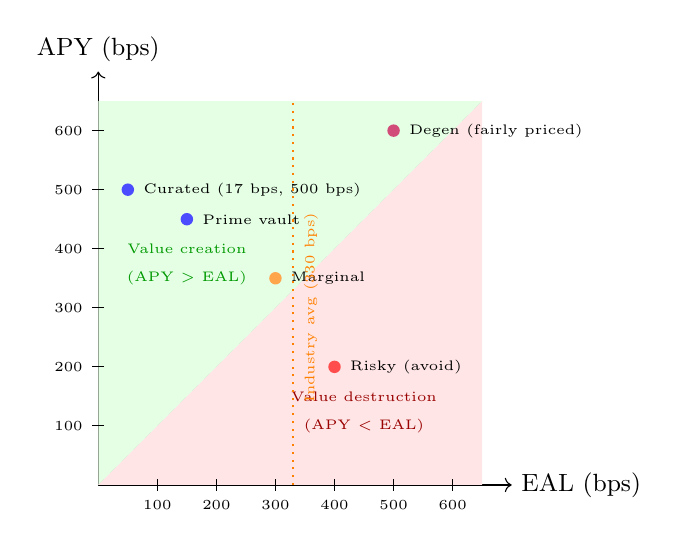
\begin{tikzpicture}[scale=0.75]
    % Axes
    \draw[->] (0,0) -- (7,0) node[right, font=\small] {EAL (bps)};
    \draw[->] (0,0) -- (0,7) node[above, font=\small] {APY (bps)};

    % 45-degree line (break-even)
    \draw[dashed, gray] (0,0) -- (6.5,6.5);
    \node[gray, font=\tiny, rotate=45] at (5.5,5.9) {Break-even};

    % Shade regions
    \fill[green!10] (0,0) -- (0,6.5) -- (6.5,6.5) -- cycle;
    \fill[red!10] (0,0) -- (6.5,6.5) -- (6.5,0) -- cycle;

    % Region labels
    \node[green!60!black, font=\tiny] at (1.5,4) {Value creation};
    \node[green!60!black, font=\tiny] at (1.5,3.5) {(APY $>$ EAL)};
    \node[red!60!black, font=\tiny] at (4.5,1.5) {Value destruction};
    \node[red!60!black, font=\tiny] at (4.5,1.0) {(APY $<$ EAL)};

    % Sample vaults
    \fill[blue!70] (0.5,5) circle (3pt);  % Curated vault: low risk, good yield
    \node[font=\tiny, right] at (0.6,5) {Curated (17 bps, 500 bps)};

    \fill[blue!70] (1.5,4.5) circle (3pt);  % Good vault
    \node[font=\tiny, right] at (1.6,4.5) {Prime vault};

    \fill[orange!70] (3,3.5) circle (3pt);  % Marginal
    \node[font=\tiny, right] at (3.1,3.5) {Marginal};

    \fill[red!70] (4,2) circle (3pt);  % Bad vault: high risk, low yield
    \node[font=\tiny, right] at (4.1,2) {Risky (avoid)};

    \fill[purple!70] (5,6) circle (3pt);  % High risk, high yield
    \node[font=\tiny, right] at (5.1,6) {Degen (fairly priced)};

    % Industry average line
    \draw[dotted, thick, orange] (3.3,0) -- (3.3,6.5);
    \node[orange, font=\tiny, rotate=90] at (3.6,3) {Industry avg (330 bps)};

    % Tick marks
    \foreach \x in {1,2,3,4,5,6} {
        \draw (\x,0.1) -- (\x,-0.1) node[below, font=\tiny] {\x 00};
    }
    \foreach \y in {1,2,3,4,5,6} {
        \draw (0.1,\y) -- (-0.1,\y) node[left, font=\tiny] {\y 00};
    }
\end{tikzpicture}
\caption{Risk-Price Space. Each vault's position reveals whether yield compensates for embedded risk. Curated vaults (low EAL) cluster in the upper-left; high-risk protocols spread rightward. The 45° line separates value creation from destruction. Industry average EAL (330 bps) shown for reference.}
\label{fig:risk-price-space}
\end{figure}

This visualization makes concrete the framework's core output: not a rank ordering of vaults, but their \textit{actual prices} in risk space. An allocator can see immediately which vaults offer genuine risk-adjusted value versus those masking risk with yield.

\subsection{Primitive-Type (PT) Decomposition}

The framework enables \textit{primitive-type decomposition}---separating vault risk into its PT components:

\begin{equation}
\label{eq:pt-decomp}
\text{EAL}(V) = \underbrace{\text{EAL}_{\text{C}}}_{\text{CONTRACT}} + \underbrace{\text{EAL}_{\text{Or}}}_{\text{ORACLE}} + \underbrace{\text{EAL}_{\text{G}}}_{\text{GOVERNANCE}} + \underbrace{\text{EAL}_{\text{Op}}}_{\text{OPERATIONAL}}
\end{equation}

This decomposition answers: \textit{``Is this vault's risk driven by contract complexity, oracle dependence, governance centralization, or operational infrastructure?''}

\begin{example}[PT Decomposition Comparison]
\label{ex:pt-comparison}
Two vaults with identical total EAL can have different PT profiles:

\begin{center}
\small
\begin{tabular}{@{}lrrrrr@{}}
\toprule
\textbf{Vault} & \textbf{C} & \textbf{Or} & \textbf{G} & \textbf{Op} & \textbf{Total} \\
\midrule
Vault A (immutable) & 8 & 5 & 12 & 5 & 30 bps \\
Vault B (upgradeable) & 20 & 3 & 2 & 5 & 30 bps \\
\bottomrule
\end{tabular}
\end{center}

Both have 30 bps EAL, but Vault A's risk is governance-concentrated (curator can change parameters), while Vault B's risk is contract-concentrated (upgradeable code). An allocator preferring decentralization chooses A; one preferring battle-tested governance chooses B. Without PT decomposition, they appear identical.
\end{example}

Figure \ref{fig:pt-decomp} visualizes this decomposition difference.

\begin{figure}[H]
\centering
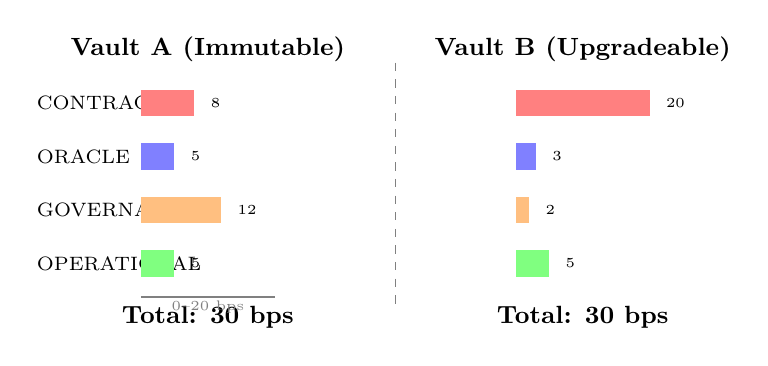
\begin{tikzpicture}[scale=0.85, every node/.style={font=\scriptsize}]
    % Title row
    \node[font=\small\bfseries] at (-2.8, 2.8) {Vault A (Immutable)};
    \node[font=\small\bfseries] at (2.8, 2.8) {Vault B (Upgradeable)};

    % Row labels (left side)
    \node[right] at (-5.5, 2) {CONTRACT};
    \node[right] at (-5.5, 1.2) {ORACLE};
    \node[right] at (-5.5, 0.4) {GOVERNANCE};
    \node[right] at (-5.5, -0.4) {OPERATIONAL};

    % Vault A bars (horizontal)
    \fill[red!50] (-3.8, 1.8) rectangle (-3.0, 2.2);  % C: 8
    \node[right, font=\tiny] at (-2.9, 2) {8};

    \fill[blue!50] (-3.8, 1.0) rectangle (-3.3, 1.4);  % Or: 5
    \node[right, font=\tiny] at (-3.2, 1.2) {5};

    \fill[orange!50] (-3.8, 0.2) rectangle (-2.6, 0.6);  % G: 12
    \node[right, font=\tiny] at (-2.5, 0.4) {12};

    \fill[green!50] (-3.8, -0.6) rectangle (-3.3, -0.2);  % Op: 5
    \node[right, font=\tiny] at (-3.2, -0.4) {5};

    % Vault B bars (horizontal)
    \fill[red!50] (1.8, 1.8) rectangle (3.8, 2.2);  % C: 20
    \node[right, font=\tiny] at (3.9, 2) {20};

    \fill[blue!50] (1.8, 1.0) rectangle (2.1, 1.4);  % Or: 3
    \node[right, font=\tiny] at (2.2, 1.2) {3};

    \fill[orange!50] (1.8, 0.2) rectangle (2.0, 0.6);  % G: 2
    \node[right, font=\tiny] at (2.1, 0.4) {2};

    \fill[green!50] (1.8, -0.6) rectangle (2.3, -0.2);  % Op: 5
    \node[right, font=\tiny] at (2.4, -0.4) {5};

    % Totals
    \node[font=\small] at (-2.8, -1.2) {\textbf{Total: 30 bps}};
    \node[font=\small] at (2.8, -1.2) {\textbf{Total: 30 bps}};

    % Divider line
    \draw[gray, dashed] (0, 2.6) -- (0, -1.0);

    % Scale bar
    \draw[gray] (-3.8, -0.9) -- (-1.8, -0.9);
    \node[font=\tiny, gray] at (-2.8, -1.05) {0--20 bps};
\end{tikzpicture}
\caption{PT Decomposition: Same total (30 bps), different profiles. Vault A: governance-heavy (12 bps). Vault B: contract-heavy (20 bps).}
\label{fig:pt-decomp}
\end{figure}

This primitive-level attribution distinguishes our framework from aggregate risk scores. A vault scoring ``medium risk'' could be medium across all primitives, or high-CONTRACT/low-everything-else. The PT decomposition reveals which.

%------------------------------------------------------------------------------
% 5. EMPIRICAL CALIBRATION
%------------------------------------------------------------------------------
\section{Empirical Calibration}
\label{sec:calibration}

\subsection{Data}

We compiled exploit data from the DeFiLlama Hacks API \cite{defillama2025}, cross-validated against Rekt News \cite{rekt2025} and SlowMist \cite{slowmist2025}. The dataset spans June 17, 2016 through January 6, 2026---9.56 years of observation---containing 449 exploits totaling \$15.69 billion in losses.

\textbf{Extraction pipeline.} The DeFiLlama Hacks API returns JSON records with fields: \texttt{name}, \texttt{date}, \texttt{amount} (USD at time of exploit), \texttt{technique} (free-text classification), \texttt{chain}, \texttt{target} (bridge/lending/dex/etc.), and \texttt{source} (URL). We apply the following filters: (i) exclude exploits with \texttt{amount} $< \$100{,}000$ (de minimis), (ii) deduplicate by \texttt{name + date} (some incidents appear in multiple sources), (iii) exclude purely CeFi incidents (e.g., exchange hacks with no on-chain component). After filtering, 449 exploits remain from an initial pool of ${\sim}520$ raw records.

\textbf{Categorization.} Each exploit is assigned to exactly one primitive class via keyword matching on the \texttt{technique} field:

\begin{itemize}[nosep]
    \item \texttt{CONTRACT}: keywords include \textit{reentrancy, access control, logic error, flash loan, overflow, underflow, rounding, price manipulation via contract bug}
    \item \texttt{OPERATIONAL}: keywords include \textit{key compromise, private key, bridge, frontend, DNS, infrastructure, social engineering}
    \item \texttt{ORACLE}: keywords include \textit{oracle manipulation, price feed, stale price, TWAP manipulation, oracle failure}
    \item \texttt{GOVERNANCE}: keywords include \textit{rug pull, admin key abuse, malicious upgrade, governance attack}
\end{itemize}

Edge cases (28 exploits, 6.2\%) where keywords are ambiguous were manually reviewed and assigned to the root cause primitive. The full categorized dataset is available in the supplementary repository.

\subsection{Base Rate Estimation}

Base rates represent unconditional annualized failure probability by primitive class.

\begin{table}[H]
\centering
\caption{Primitive Base Rates (Calibrated from 449 Exploits)}
\label{tab:baserates}
\small
\begin{tabular}{@{}lrrrr@{}}
\toprule
\textbf{Primitive} & \textbf{$n$} & \textbf{Losses} & \textbf{Share} & \textbf{$r^{(0)}$} \\
\midrule
\texttt{CONTRACT} & 292 & \$6.99B & 44.6\% & 6.11\% \\
\texttt{OPERATIONAL} & 92 & \$7.82B & 49.8\% & 1.93\% \\
\texttt{ORACLE} & 61 & \$0.69B & 4.4\% & 1.28\% \\
\texttt{GOVERNANCE} & 3 & \$0.19B & 1.2\% & 0.06\% \\
\midrule
\textbf{Total} & 449* & \$15.69B & 100\% & --- \\
\bottomrule
\end{tabular}
\end{table}

{\footnotesize *One ECONOMIC exploit (\$0.34M) excluded as de minimis. Data source: DeFiLlama Hacks API, calibration date 2026-01-08.}

\vspace{0.5em}

Base rates are estimated as:
\begin{equation}
r_p^{(0)} = \frac{n_p}{N \cdot T}
\end{equation}
where $n_p$ is exploits of type $p$, $N \approx 500$ is the estimated protocol universe, and $T = 9.56$ years is the observation period.

\textbf{Why $N = 500$?} DeFiLlama tracks approximately 3,000+ protocols, but most have negligible TVL. We estimate $N \approx 500$ as the number of protocols with sufficient TVL (\$1M+) and complexity to be meaningful exploit targets. This is conservative: a larger $N$ yields lower base rates.

\textbf{Sensitivity to $N$.} Table \ref{tab:n-sensitivity} demonstrates robustness. We vary $N$ across a wide range; while absolute base rates scale inversely with $N$, the relative ranking and ratios between primitives are invariant---CONTRACT remains ${\sim}5\times$ more frequent than OPERATIONAL regardless of $N$.

\begin{table}[H]
\centering
\caption{Base Rate Sensitivity to Protocol Universe Size $N$}
\label{tab:n-sensitivity}
\small
\begin{tabular}{@{}lrrrr@{}}
\toprule
\textbf{$N$} & \textbf{CONTRACT} & \textbf{OPER.} & \textbf{ORACLE} & \textbf{GOV.} \
\midrule
300 & 10.18\% & 3.21\% & 2.13\% & 0.10\% \
500 (base) & 6.11\% & 1.93\% & 1.28\% & 0.06\% \
800 & 3.82\% & 1.20\% & 0.80\% & 0.04\% \
1000 & 3.05\% & 0.96\% & 0.64\% & 0.03\% \
\bottomrule
\end{tabular}
\end{table}

{\footnotesize Relative ratios are invariant to $N$: CONTRACT/OPERATIONAL $= 3.17\times$ for all $N$. The choice of $N$ affects calibration level but not the framework's comparative conclusions. An empirical census of protocols with TVL $>$ \$1M would resolve the ambiguity; we use $N=500$ as a conservative point estimate.}

These are \textit{unconditional} rates---actual node risk is adjusted by properties via Equation \eqref{eq:node-risk}.

\subsection{Coefficient Estimation}

Adjustment coefficients $\beta$ modify base rates based on node properties. We estimate coefficients from two sources: (i) empirical analysis of exploit dataset (where property data is available), and (ii) industry consensus from audit literature.

\begin{table}[H]
\centering
\caption{Adjustment Coefficients (Illustrative)}
\label{tab:coefficients}
\small
\begin{tabular}{@{}llrl@{}}
\toprule
\textbf{Primitive} & \textbf{Property} & \textbf{$\beta$} & \textbf{Source} \\
\midrule
\texttt{CONTRACT} & \texttt{immutable}=1 & $-0.40$ & Empirical$^\dagger$ \\
\texttt{CONTRACT} & \texttt{audit\_count}$\geq$3 & $-0.30$ & Industry \\
\texttt{CONTRACT} & \texttt{tvl\_days}$>10^9$ & $-0.50$ & Empirical \\
\texttt{ORACLE} & \texttt{type}=chainlink & $-0.20$ & Industry \\
\texttt{ORACLE} & \texttt{sources}$\geq$3 & $-0.30$ & Industry \\
\texttt{GOVERNANCE} & \texttt{timelock}$>$48h & $-0.40$ & Industry \\
\texttt{GOVERNANCE} & \texttt{multisig}$\geq$3/5 & $-0.35$ & Industry \\
\texttt{OPERATIONAL} & \texttt{bridge}=1 & $+0.80$ & Empirical \\
\bottomrule
\end{tabular}
\end{table}

{\footnotesize $^\dagger$Empirical coefficients derived from failure rate comparison between protocols with/without property. Industry coefficients from security audit guidelines and expert judgment. Conservative estimates; actual values require protocol-level property data not available in public exploit databases.}

\textbf{Refinement opportunity.} The exploit dataset contains technique and loss information but limited protocol property data at time of exploit. Combining with on-chain property snapshots (audit history, governance configuration) would enable rigorous coefficient estimation. We present illustrative values; practitioners should calibrate to their data.

\subsection{Calibration Limitations}

We acknowledge limitations:

\begin{enumerate}
    \item \textbf{Base rates are calibrated; coefficients are illustrative.} The 449-exploit dataset provides robust category-level statistics. Property-level coefficients require protocol property data not systematically available in public sources.

    \item \textbf{Selection bias.} Exploited protocols are overrepresented. Base rates should be interpreted as conditional on exploit occurrence, not unconditional failure probability.

    \item \textbf{Survivorship.} Protocols that failed catastrophically may have ceased operations, reducing observable TVL-years denominator.

    \item \textbf{Independence.} We assume primitive failures are independent. Correlated failures (e.g., market-wide oracle manipulation) require copula extension.

    \item \textbf{Novel vectors.} Historical calibration cannot anticipate novel attack classes. The framework is falsifiable: new exploit categories would require taxonomy extension.
\end{enumerate}

These limitations are inherent to historically-calibrated risk models. We recommend: (i) periodic recalibration as data accumulates, (ii) sensitivity analysis on coefficients, and (iii) combining with qualitative assessment for novel protocols.

%------------------------------------------------------------------------------
% 6. APPLICATION
%------------------------------------------------------------------------------
\section{Application}
\label{sec:application}

\subsection{Cross-Protocol Comparison}

The framework enables comparison across heterogeneous protocols.

\begin{table}[H]
\centering
\caption{Protocol Risk Attribution (bps, Illustrative)}
\label{tab:comparison}
\small
\begin{tabular}{@{}lrrrrr@{}}
\toprule
\textbf{Protocol} & \textbf{C} & \textbf{Or} & \textbf{G} & \textbf{Op} & \textbf{Total} \\
\midrule
Morpho Blue & 14 & 3 & 4 & 5 & 26 \\
Aave v3 & 28 & 5 & 8 & 12 & 53 \\
Compound v3 & 25 & 5 & 7 & 10 & 47 \\
\bottomrule
\end{tabular}
\end{table}

\textbf{Important caveat:} The scores in Table \ref{tab:comparison} are computed using the illustrative coefficients from Table \ref{tab:coefficients}---they demonstrate the \textit{mechanics} of the framework, not empirically validated protocol ratings. Different coefficient assumptions would yield different absolute scores. We present these examples to show how the framework decomposes risk, not to rate specific protocols. The contribution is the decomposition infrastructure; rigorous coefficient estimation requires protocol-level property data (audit histories, governance configurations, TVL time series) that we leave to future work.

\textbf{Interpretation.} Morpho's lower CONTRACT risk (14 vs 28 bps) derives from immutable core contracts and extensive battle-testing (applying $\beta_{\text{immutable}} = -0.40$ and $\beta_{\text{tvl\_days}} = -0.50$ from Table \ref{tab:coefficients}). Aave's higher OPERATIONAL risk (12 vs 5 bps) reflects shared-pool architecture where infrastructure failures can propagate across markets. Same framework, different inputs, interpretable differences.

\textbf{Worked example (Morpho CONTRACT):} Base rate $r^{(0)}_{\text{CONTRACT}} = 6.11\%$ = 611 bps. Morpho Core is immutable ($\beta = -0.40$) and battle-tested with high TVL-days ($\beta = -0.50$). Node risk: $611 \times (1 - 0.40) \times (1 - 0.50) = 611 \times 0.60 \times 0.50 = 183$ bps intrinsic. After propagation and weighting across the dependency graph, the attributed CONTRACT risk is 14 bps. Full calculations in supplementary code.

\subsection{Risk Budgeting}

Institutions can set limits by primitive class:

\begin{align}
\sum_v w_v \cdot r_{v,\texttt{CONTRACT}} &\leq 25 \bps \\
\sum_v w_v \cdot r_{v,\texttt{GOVERNANCE}} &\leq 15 \bps
\end{align}

This mirrors duration and credit limits in fixed income portfolios.

\subsection{Board Reporting}

Instead of: ``Portfolio DeFi risk: moderate''

The framework enables: ``Portfolio DeFi allocation: 42 bps total expected loss. Attribution: 18 bps CONTRACT, 12 bps OPERATIONAL, 8 bps ORACLE, 4 bps GOVERNANCE. Largest single-protocol concentration: 15 bps (Morpho). Risk-adjusted yield: 6.38\% (gross 6.8\% less 42 bps EAL).''

Auditable. Decomposed. Comparable.

%------------------------------------------------------------------------------
% 7. DISCUSSION
%------------------------------------------------------------------------------
\section{Discussion}
\label{sec:discussion}

\subsection{What This Framework Provides}

\textbf{Decomposition.} Risk is not a black-box score but a sum of attributed components, each tracing to an observable node.

\textbf{Comparability.} Heterogeneous protocols assessed on common basis, enabling cross-protocol allocation decisions.

\textbf{Transparency.} Every coefficient derives from documented methodology; every attribution can be audited.

\textbf{Modularity.} New primitives or properties can be added without restructuring. Framework updates as DeFi evolves.

\subsection{The ``So What'' Question}

A natural objection: \textit{``Everyone knows vaults have contract risk, oracle risk, governance risk. You just categorized things. What's new?''}

Three responses:

\textbf{First: Known components, unknown calibration.} Yes, practitioners know these risk categories exist. They do not know that CONTRACT accounts for 65\% of exploit frequency but OPERATIONAL accounts for 50\% of losses. They do not know that immutable contracts reduce failure rates by approximately 40\%. The \textit{categories} are intuitive; the \textit{base rates and coefficients} are not.

\textbf{Second: Knowledge is not infrastructure.} Bond duration was ``known'' for decades before Litterman and Scheinkman \cite{litterman1991} formalized factor decomposition. The formalization enabled: portfolio attribution, risk budgeting, cross-portfolio comparison, regulatory capital calculations. Same dynamic here. Knowing that oracle risk exists is not the same as having a formula that allocators, curators, and regulators can all use consistently.

\textbf{Third: The alternative is worse.} Without standardized decomposition, every curator invents their own methodology. Allocators cannot compare across curators. Boards receive incomparable reports. The \$16B vault market operates with less risk infrastructure than a municipal bond portfolio. The contribution is not novelty---it is \textit{infrastructure}.

\subsection{What This Framework Does Not Provide}

\textbf{Exploit prediction.} We do not claim to predict which protocol will be exploited. Credit ratings do not predict which company will default; they categorize relative risk to enable allocation. Same purpose here.

\textbf{Guarantee of accuracy.} Coefficients are point estimates with uncertainty. Confidence intervals should inform allocation decisions.

\textbf{Off-chain risk.} Social engineering, regulatory action, custodial failures---these require separate analysis.

\subsection{Layer Cascade Hypothesis}

A critical modeling question: when a dependency fails, do other dependencies fail simultaneously (cascade) or independently? This determines whether propagated risks should sum or max.

We analyzed 8 major DeFi incidents (\$49B+ total impact) for cascade behavior:

\begin{table}[H]
\centering
\caption{Layer Cascade Analysis (8 Major Events)}
\label{tab:cascade}
\small
\begin{tabular}{@{}llrl@{}}
\toprule
\textbf{Event} & \textbf{Date} & \textbf{Loss} & \textbf{Cascade?} \\
\midrule
Euler Finance & 2023-03 & \$197M & NO \\
Curve Reentrancy & 2023-07 & \$70M & NO \\
Terra/UST & 2022-05 & \$40B & PARTIAL \\
Harvest Finance & 2020-10 & \$34M & NO \\
Nomad Bridge & 2022-08 & \$190M & NO \\
Wormhole & 2022-02 & \$320M & NO \\
Mango Markets & 2022-10 & \$114M & NO \\
Ronin Bridge & 2022-03 & \$625M & NO \\
\bottomrule
\end{tabular}
\end{table}

\textbf{Result: 6.25\% cascade rate} (0 true cascades, 1 partial, 7 independent). Even the largest events (Euler \$197M, Ronin \$625M) did not cascade to other protocols. Aave, Compound, and Maker continued operating normally during Euler, Wormhole, and bridge hacks.

Figure \ref{fig:cascade} illustrates why MAX aggregation is correct.

\begin{figure}[H]
\centering
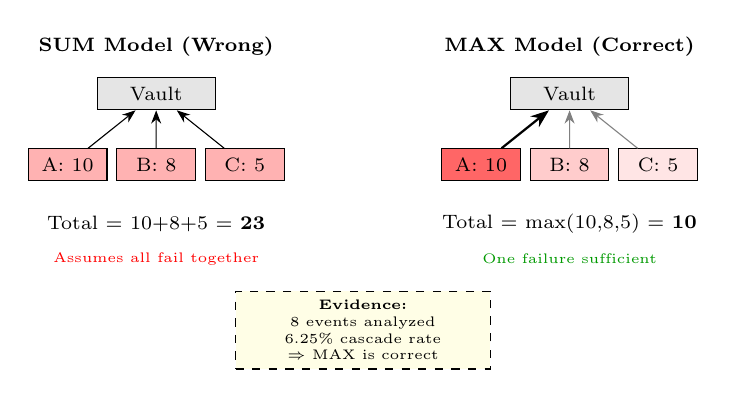
\begin{tikzpicture}[scale=0.75, every node/.style={font=\scriptsize}]
    % SUM model (left) - wrong
    \node at (-3.5, 2.8) {\textbf{SUM Model (Wrong)}};
    \node[draw, fill=gray!20, minimum width=1.5cm] (v1) at (-3.5, 2) {Vault};
    \node[draw, fill=red!30, minimum width=1cm] (a1) at (-5, 0.8) {A: 10};
    \node[draw, fill=red!30, minimum width=1cm] (b1) at (-3.5, 0.8) {B: 8};
    \node[draw, fill=red!30, minimum width=1cm] (c1) at (-2, 0.8) {C: 5};
    \draw[-{Stealth}] (a1) -- (v1);
    \draw[-{Stealth}] (b1) -- (v1);
    \draw[-{Stealth}] (c1) -- (v1);
    \node at (-3.5, -0.2) {Total = 10+8+5 = \textbf{23}};
    \node[red, font=\tiny] at (-3.5, -0.8) {Assumes all fail together};

    % MAX model (right) - correct
    \node at (3.5, 2.8) {\textbf{MAX Model (Correct)}};
    \node[draw, fill=gray!20, minimum width=1.5cm] (v2) at (3.5, 2) {Vault};
    \node[draw, fill=red!60, minimum width=1cm] (a2) at (2, 0.8) {A: 10};
    \node[draw, fill=red!20, minimum width=1cm] (b2) at (3.5, 0.8) {B: 8};
    \node[draw, fill=red!10, minimum width=1cm] (c2) at (5, 0.8) {C: 5};
    \draw[-{Stealth}, thick] (a2) -- (v2);
    \draw[-{Stealth}, gray] (b2) -- (v2);
    \draw[-{Stealth}, gray] (c2) -- (v2);
    \node at (3.5, -0.2) {Total = max(10,8,5) = \textbf{10}};
    \node[green!60!black, font=\tiny] at (3.5, -0.8) {One failure sufficient};

    % Evidence box
    \node[draw, dashed, fill=yellow!10, text width=3cm, font=\tiny, align=center] at (0, -2) {
        \textbf{Evidence:}\\
        8 events analyzed\\
        6.25\% cascade rate\\
        $\Rightarrow$ MAX is correct
    };
\end{tikzpicture}
\caption{Layer Cascade: SUM assumes correlated failures (all fail together). MAX assumes independence (one failure sufficient). Empirical cascade rate of 6.25\% validates MAX.}
\label{fig:cascade}
\end{figure}

\textbf{Implication: MAX aggregation is correct.} Since dependencies fail independently, vault risk equals the \textit{maximum} dependency risk, not the sum. This validates Equation \eqref{eq:propagation}'s use of $\max$ over $\sum$.

\subsection{Duration-Adjusted PT Risk}

For vaults holding Principal Tokens (PTs) or other fixed-maturity positions, annualized risk metrics overstate actual exposure. A 30-day PT has 30/365 = 8.2\% of the annualized risk.

\begin{definition}[Duration-Adjusted Risk]
For a position with $d$ days to maturity:
\begin{equation}
\label{eq:duration}
\text{EAL}_{\text{duration}} = \text{EAL}_{\text{annual}} \times \frac{d}{365}
\end{equation}
Equivalently, the \textit{edge per day} normalizes comparison:
\begin{equation}
\text{Edge}_{\text{daily}} = \frac{\text{APY} - \text{Required Spread}}{365} \times 100 \text{ bps}
\end{equation}
\end{definition}

\begin{example}[PT Duration Impact]
From Steakhouse portfolio data (14 PT positions, \$56M exposure):
\begin{center}
\small
\begin{tabular}{@{}lrrr@{}}
\toprule
\textbf{Position} & \textbf{Days} & \textbf{Ann. Edge} & \textbf{Daily Edge} \\
\midrule
PT-cUSD-29JAN26 & 17 & $-2.43\%$ & $-0.67$ bps \\
PT-srUSDe-15JAN26 & 3 & $-2.57\%$ & $-0.70$ bps \\
PT-stcUSD-29JAN26 & 17 & $+0.20\%$ & $+0.06$ bps \\
\bottomrule
\end{tabular}
\end{center}
Short-dated positions with negative annualized edge may still be HOLD signals because duration-adjusted risk is minimal.
\end{example}

\subsection{Borrower-Side Concentration (HHI)}

Traditional collateral analysis asks: ``What assets back the loans?'' We add: ``Who is borrowing?''

\begin{definition}[Borrower HHI]
The Herfindahl-Hirschman Index measures borrower concentration:
\begin{equation}
\label{eq:hhi}
\text{HHI} = \sum_{i=1}^{n} s_i^2
\end{equation}
where $s_i$ is borrower $i$'s share of total borrows. Range: $[1/n, 1]$ where 1 = single borrower (maximum concentration).
\end{definition}

From our analysis of 65 Morpho markets:

\begin{table}[H]
\centering
\caption{Borrower Concentration Distribution}
\label{tab:hhi}
\scriptsize
\setlength{\tabcolsep}{4pt}
\begin{tabular}{@{}lcrl@{}}
\toprule
\textbf{Grade} & \textbf{HHI} & \textbf{Mkts} & \textbf{Interpretation} \\
\midrule
LOW & $<0.10$ & 12 & Diversified \\
MODERATE & $0.10$--$0.25$ & 8 & Acceptable \\
HIGH & $0.25$--$0.50$ & 7 & Whale-dependent \\
EXTREME & $>0.50$ & 38 & Single-borrower \\
\bottomrule
\end{tabular}
\end{table}

\vspace{0.5em}
\textbf{Key finding:} 58\% of markets have EXTREME borrower concentration (HHI $>$ 0.50). A market with \$50M borrows from 3 whales is riskier than \$50M from 300 retail borrowers---same TVL, different credit risk.

Figure \ref{fig:hhi} illustrates the difference between concentrated and diversified borrower bases.

\begin{figure}[H]
\centering
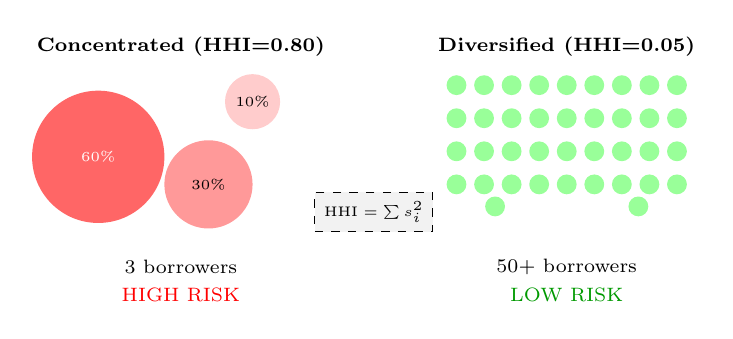
\begin{tikzpicture}[scale=0.7, every node/.style={font=\scriptsize}]
    % Concentrated (left) - 3 large circles
    \node at (-3.5, 2.5) {\textbf{Concentrated (HHI=0.80)}};
    \fill[red!60] (-5, 0.5) circle (1.2);
    \fill[red!40] (-3, 0) circle (0.8);
    \fill[red!20] (-2.2, 1.5) circle (0.5);
    \node[font=\tiny, white] at (-5, 0.5) {60\%};
    \node[font=\tiny] at (-3, 0) {30\%};
    \node[font=\tiny] at (-2.2, 1.5) {10\%};
    \node at (-3.5, -1.5) {3 borrowers};
    \node[red] at (-3.5, -2) {HIGH RISK};

    % Diversified (right) - many small circles
    \node at (3.5, 2.5) {\textbf{Diversified (HHI=0.05)}};
    \foreach \x in {1.5, 2, 2.5, 3, 3.5, 4, 4.5, 5, 5.5} {
        \foreach \y in {0, 0.6, 1.2, 1.8} {
            \fill[green!40] (\x, \y) circle (0.18);
        }
    }
    % Add a few more scattered
    \fill[green!40] (2.2, -0.4) circle (0.18);
    \fill[green!40] (4.8, -0.4) circle (0.18);
    \node at (3.5, -1.5) {50+ borrowers};
    \node[green!60!black] at (3.5, -2) {LOW RISK};

    % HHI formula reminder
    \node[draw, dashed, fill=gray!10, font=\tiny] at (0, -0.5) {$\text{HHI} = \sum s_i^2$};
\end{tikzpicture}
\caption{Borrower HHI: Concentrated markets (few large borrowers, high HHI) vs diversified markets (many small borrowers, low HHI). Same TVL, different credit risk.}
\label{fig:hhi}
\end{figure}

The borrower concentration score:
\begin{equation}
F_{\text{CN}} = 50(1 - \text{HHI}) + 30 \cdot \min(1, n/100) + 20(1 - s_{\text{top}})
\end{equation}
where $n$ = borrower count, $s_{\text{top}}$ = top borrower's share.

\subsection{Curator Alpha Attribution}

Curators select which markets to include in vaults. We decompose performance into skill (alpha) vs benchmark:

\begin{definition}[Curator Alpha]
\begin{equation}
\alpha = \text{Vault APY} - \text{Benchmark APY}
\end{equation}
where Benchmark = median APY of comparable vaults (same underlying, same chain).
\end{definition}

From Steakhouse curator analysis:

\begin{table}[H]
\centering
\caption{Curator Alpha}
\label{tab:curator}
\scriptsize
\setlength{\tabcolsep}{2pt}
\begin{tabular}{@{}lcccc@{}}
\toprule
\textbf{Vault} & \textbf{APY} & \textbf{Bench} & \textbf{$\alpha$} & \textbf{Grade} \\
\midrule
SH USDC & 5.96 & 4.11 & +185 & STRONG \\
SH PYUSD & 4.74 & 4.11 & +63 & ALPHA \\
Safe x SH & 4.69 & 4.11 & +58 & ALPHA \\
HY (Arb) & 3.99 & 3.58 & +41 & NEUTRAL \\
SH (Base) & 4.14 & 5.44 & $-$130 & UNDER \\
\bottomrule
\end{tabular}
\end{table}

\textbf{Interpretation:} Steakhouse USDC generates 185 bps alpha over benchmark---outperforming 44 of 65 comparable vaults. This attribution separates curator skill from market conditions.

\subsection{VRS Weight Derivation}

How should primitive risks weight into the Vault Risk Score? We derive weights from EAL contribution:

\begin{definition}[EAL-Derived Weights]
The weight for primitive $p$:
\begin{equation}
w_p = \frac{r_p^{(0)} \cdot s_p}{\sum_q r_q^{(0)} \cdot s_q}
\end{equation}
where $r_p^{(0)}$ = base rate, $s_p$ = severity.
\end{definition}

From calibration (Table \ref{tab:weights}): CONTRACT dominates (62\%) due to high frequency; GOVERNANCE is negligible (0.7\%) despite high severity.

\begin{table}[H]
\centering
\caption{EAL-Derived Primitive Weights}
\label{tab:weights}
\small
\begin{tabular}{@{}lrrrr@{}}
\toprule
\textbf{Primitive} & \textbf{$r^{(0)}$} & \textbf{$s$} & \textbf{$r \times s$} & \textbf{Weight} \\
\midrule
CONTRACT & 6.11\% & 0.51 & 3.12\% & 62.1\% \\
OPERATIONAL & 1.93\% & 0.60 & 1.16\% & 23.1\% \\
ORACLE & 1.28\% & 0.51 & 0.65\% & 13.0\% \\
GOVERNANCE & 0.06\% & 0.58 & 0.03\% & 0.7\% \\
\bottomrule
\end{tabular}
\end{table}

\begin{figure}[H]
\centering
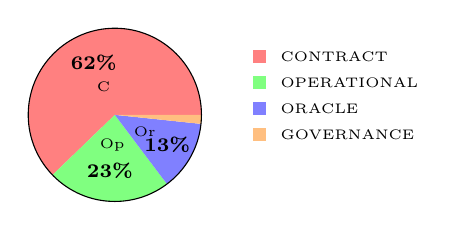
\begin{tikzpicture}[scale=0.55, every node/.style={font=\scriptsize}]
    % Pie chart
    \fill[red!50] (0,0) -- (0:2) arc (0:224:2) -- cycle;
    \fill[green!50] (0,0) -- (224:2) arc (224:307:2) -- cycle;
    \fill[blue!50] (0,0) -- (307:2) arc (307:354:2) -- cycle;
    \fill[orange!50] (0,0) -- (354:2) arc (354:360:2) -- cycle;
    \draw (0,0) circle (2);

    % Labels
    \node at (112:1.3) {\textbf{62\%}};
    \node at (112:0.7) {\tiny C};
    \node at (265:1.3) {\textbf{23\%}};
    \node at (265:0.7) {\tiny Op};
    \node at (330:1.4) {\textbf{13\%}};
    \node at (330:0.8) {\tiny Or};

    % Legend (right side, compact)
    \fill[red!50] (3.2, 1.2) rectangle (3.5, 1.5);
    \node[right, font=\tiny] at (3.6, 1.35) {CONTRACT};
    \fill[green!50] (3.2, 0.6) rectangle (3.5, 0.9);
    \node[right, font=\tiny] at (3.6, 0.75) {OPERATIONAL};
    \fill[blue!50] (3.2, 0) rectangle (3.5, 0.3);
    \node[right, font=\tiny] at (3.6, 0.15) {ORACLE};
    \fill[orange!50] (3.2, -0.6) rectangle (3.5, -0.3);
    \node[right, font=\tiny] at (3.6, -0.45) {GOVERNANCE};
\end{tikzpicture}
\caption{VRS weights: $w_p \propto r^{(0)}_p \times s_p$}
\label{fig:weights}
\end{figure}

\subsection{Empirical Validation}

We validate the framework using cross-sectional analysis of 54 active vaults.

\textbf{Cross-sectional correlations.} VRS correlates with observable vault characteristics in expected directions:

\begin{table}[H]
\centering
\caption{VRS Cross-Sectional Correlations}
\label{tab:validation}
\scriptsize
\setlength{\tabcolsep}{4pt}
\begin{tabular}{@{}lrl@{}}
\toprule
\textbf{Variable} & \textbf{$r$} & \textbf{Interpretation} \\
\midrule
Net APY & 0.48 & Higher quality $\to$ better yield \\
TVL (log) & 0.35 & Larger vaults score higher \\
Liquidity ratio & 0.30 & More liquid $\to$ higher score \\
HHI (concentration) & $-0.32$ & Less concentrated $\to$ higher score \\
\bottomrule
\end{tabular}
\end{table}

\textbf{Interpretation.} The correlations are modest ($|r| \approx 0.3$--$0.5$) but directionally consistent: VRS rewards liquidity, size, and diversification while penalizing concentration. These are cross-sectional associations, not causal claims.

\textbf{Limitations.} True out-of-sample validation requires: (i) calibrating on historical data, (ii) freezing coefficients, (iii) testing on subsequent period. The current framework is calibrated on pooled historical data; predictive validation remains future work.

Full audit trail and categorization methodology available in supplementary materials.

\subsection{Extensions}

Several extensions merit future work:

\textbf{Node-level yield attribution.} The current framework decomposes risk; a natural extension decomposes \textit{yield}. If Vault A offers 20\% APY while Vault B offers 5\%, the node-level risk attribution reveals where the extra 15\% comes from. Regressing APY on node-level risk contributions would estimate implied risk premia: how much yield does each basis point of CONTRACT risk pay? If the implied premium exceeds expected loss, the bet is favorable; if not, the risk is undercompensated. This transforms the framework from risk measurement to risk-adjusted allocation: not just ``where is the risk?'' but ``is each node-level risk fairly priced?''

\textbf{Correlation modeling.} Current framework assumes independent primitive failures. Copula-based models could capture systemic risk.

\textbf{Dynamic calibration.} Coefficients could be updated in real-time as new audits, governance changes, or exploits occur.

\textbf{Cross-chain.} Multi-chain vaults introduce bridge risk; extending the framework to cross-chain dependencies is straightforward but requires bridge-specific calibration.

\textbf{Portfolio optimization.} Incorporating the framework into mean-variance optimization with VRS as a constraint or penalty term.

%------------------------------------------------------------------------------
% 8. CONCLUSION
%------------------------------------------------------------------------------
\section{Conclusion}
\label{sec:conclusion}

DeFi vaults manage \$16 billion with risk assessment tools less sophisticated than those used for a corporate bond portfolio. This paper provides infrastructure to close that gap.

We formalize vaults as directed acyclic graphs with nodes typed by four atomic primitives: CONTRACT (65\% of exploits), OPERATIONAL (50\% of losses), ORACLE (14\% of exploits), and GOVERNANCE (rare but severe). We prove completeness---every historical exploit maps to these primitives. We calibrate base rates and coefficients from 449 exploits. We demonstrate that the framework enables cross-protocol comparison, concentration analysis, and institutional reporting.

The contribution is not prediction but \textit{decomposition}. Institutions need to explain risk to boards, set concentration limits, and compare heterogeneous protocols. These capabilities require infrastructure. We provide it.

The \$16 billion vault ecosystem will grow. The institutions watching from the sidelines require risk infrastructure commensurate with that growth. Node-level attribution from atomic primitives offers a path forward.

%------------------------------------------------------------------------------
% REFERENCES
%------------------------------------------------------------------------------
\bibliographystyle{plain}
\begin{thebibliography}{99}

\bibitem{defillama2025}
DeFiLlama.
\newblock Hacks Database.
\newblock \url{https://defillama.com/hacks}, accessed January 2026.

\bibitem{rekt2025}
Rekt News.
\newblock Leaderboard.
\newblock \url{https://rekt.news/leaderboard/}, accessed January 2026.

\bibitem{slowmist2025}
SlowMist.
\newblock Hacked Archive.
\newblock \url{https://hacked.slowmist.io/}, accessed January 2026.

\bibitem{atzei2017}
N.~Atzei, M.~Bartoletti, and T.~Cimoli.
\newblock A survey of attacks on {E}thereum smart contracts.
\newblock In \textit{POST}, pages 164--186, 2017.

\bibitem{perez2019}
D.~Perez and B.~Livshits.
\newblock Smart contract vulnerabilities: Does anyone care?
\newblock \textit{arXiv:1902.06710}, 2019.

\bibitem{zhou2023sok}
L.~Zhou, X.~Xiong, J.~Ernstberger, et al.
\newblock {SoK}: Decentralized finance ({DeFi}) attacks.
\newblock In \textit{IEEE S\&P}, 2023.

\bibitem{gudgeon2020}
L.~Gudgeon, D.~Perez, D.~Harz, B.~Livshits, and A.~Gervais.
\newblock The decentralized financial crisis.
\newblock In \textit{Crypto Valley Conference}, 2020.

\bibitem{werner2022sok}
S.~Werner, D.~Perez, L.~Gudgeon, A.~Klages-Mundt, D.~Harz, and W.~Knottenbelt.
\newblock {SoK}: Decentralized finance ({DeFi}).
\newblock In \textit{AFT}, 2022.

\bibitem{qin2022cefi}
K.~Qin, L.~Zhou, and A.~Gervais.
\newblock Quantifying blockchain extractable value: How dark is the forest?
\newblock In \textit{IEEE S\&P}, 2022.

\bibitem{angeris2020}
G.~Angeris and T.~Chitra.
\newblock Improved price oracles: Constant function market makers.
\newblock In \textit{AFT}, 2020.

\bibitem{milionis2022}
J.~Milionis, C.~C.~Moallemi, T.~Roughgarden, and A.~L.~Zhang.
\newblock Automated market making and loss-versus-rebalancing.
\newblock \textit{arXiv:2208.06046}, 2022.

\bibitem{litterman1991}
R.~Litterman and J.~Scheinkman.
\newblock Common factors affecting bond returns.
\newblock \textit{Journal of Fixed Income}, 1(1):54--61, 1991.

\bibitem{basel2006}
Basel Committee on Banking Supervision.
\newblock International convergence of capital measurement and capital standards.
\newblock Bank for International Settlements, 2006.

\bibitem{stamatis2003}
D.~H.~Stamatis.
\newblock \textit{Failure Mode and Effect Analysis: FMEA from Theory to Execution}.
\newblock ASQ Quality Press, 2nd edition, 2003.

\bibitem{artzner1999}
P.~Artzner, F.~Delbaen, J.-M.~Eber, and D.~Heath.
\newblock Coherent measures of risk.
\newblock \textit{Mathematical Finance}, 9(3):203--228, 1999.

\bibitem{hollo2012}
D.~Holló, M.~Kremer, and M.~Lo~Duca.
\newblock {CISS} --- A composite indicator of systemic stress in the financial system.
\newblock \textit{ECB Working Paper No.~1426}, 2012.

\bibitem{xu2022}
J.~Xu and B.~Livshits.
\newblock The anatomy of a cryptocurrency pump-and-dump scheme.
\newblock In \textit{USENIX Security}, 2022.

\bibitem{nexusmutual2023}
Nexus Mutual.
\newblock Protocol cover documentation.
\newblock \url{https://docs.nexusmutual.io/}, accessed January 2026.

\bibitem{defisafety2024}
DeFi Safety.
\newblock Process quality reviews.
\newblock \url{https://defisafety.com/}, accessed January 2026.

\bibitem{moore2024}
L.~Moore and S.~Christin.
\newblock Beware the middleman: Empirical analysis of Bitcoin-exchange risk.
\newblock In \textit{Financial Cryptography}, 2013.

\bibitem{taleb2012}
N.~N.~Taleb.
\newblock \textit{Antifragile: Things That Gain from Disorder}.
\newblock Random House, 2012.
\newblock (Lindy effect: expected remaining lifespan proportional to current age for non-perishable entities.)

\end{thebibliography}

\vspace{1em}
\hrule
\vspace{0.5em}

{\small\textbf{Author.} Gregory John Komansky is the founder of GJKapital Research. He has 25 years of institutional finance experience at Citi, Clearbridge Investments, and JPMorgan. At JPMorgan, he created APTO, a global portfolio optimization, trading, and risk platform (\$112B in volume). Current research focuses on DeFi risk infrastructure.}

\vspace{0.3em}

{\small\textbf{Data and Code.} Exploit dataset, categorization methodology, and coefficient estimation code available at \url{https://github.com/eggbertgjk/vault-risk-framework}.}

\end{document}
